\documentclass[11pt,a4paper]{article}

\usepackage{../../templates/style}

\begin{document}

\begin{problem}{ฝ่าเขาวงกต (maze)}{standard input}{standard output}{1 second}{32 megabytes}


นักล่าขุมทรัพย์นามว่า \textit{“อินเดียนา เจ”} พลาดพลั้งตกลงไปในหลุมพรางที่ส่งเขาไปอยู่ในเขาวงกตซึ่งมีทางออกอยู่เพียงตำแหน่งเดียวเท่านั้น  เคราะห์ดีที่นายอินเดียนามีแผนที่เขาวงกตติดตัวมาด้วย ทำให้เขาทราบตำแหน่งปัจจุบันของเขาและตำแหน่งของทางออก  จากแผนที่ อินเดียนาพบว่าพื้นที่เขาวงกตถูกแบ่งออกเป็นช่องจำนวน $M$ แถว $N$ หลัก โดยแต่ละช่องในแผนที่จะมีเลขหนึ่งหรือเลขศูนย์อย่างใดอย่างหนึ่ง ซึ่งเลขศูนย์แทนกำแพงและเลขหนึ่งแทนทางเดิน นอกจากนี้เขาวงกตยังวางตัวในทิศเหนือ-ใต้ ตะวันออก-ตะวันตกพอดี
ดังแสดงในภาพตัวอย่างที่อยู่หน้าถัดไป

อย่างไรก็ตามปัญหาหนักใจมีอยู่ว่า บริเวณที่อินเดียนาตกลงมาไม่ได้เชื่อมต่อกับทางออก อินเดียนาจึงจำเป็นที่จะต้องระเบิดกำแพงเขาวงกตด้วยระเบิดที่มีติดตัวอยู่เพียงลูกเดียวเท่านั้น นอกจากนี้อินเดียนาทราบว่าระเบิดนี้มีพลังทำลายกำแพงเขาวงกตได้เพียงหนึ่ง ช่องเท่านั้น

          อินเดียนา จึงจำเป็นที่จะต้องวางแผนว่าเขาจะต้องเดินในเขาวงกตอย่างไร และใช้ระเบิดทำลายกำแพงตรงพื้นที่ช่องใด จึงจะสามารถเดินไปถึงทางออกได้  อินเดียนาทราบ ตำแหน่งเริ่มต้นของเขาและตำแหน่งทางออกเท่านั้น และเพื่อให้การวางแผนและประมาณระยะทางเดินเป็นไปโดยง่าย อินเดียนาจะเดินในทิศเหนือ ใต้ ตะวันออก หรือ ตะวันตก เท่านั้น อินเดียนาจะไม่เดินในทิศเฉียงเป็นอันขาด (เช่น ไม่เดินในทิศตะวันออกเฉียงเหนือ เป็นต้น)

\textbf{ยกตัวอย่าง}จากแผนที่ด้านล่าง เขาวงกตนี้ประกอบด้วยช่องจำนวนทั้งหมด $5$ แถวและ $8$ หลัก กำหนดให้อินเดียนาเริ่มต้นในช่องที่ถูกเน้นด้วยวงรี และทางออกอยู่ ณ ตำแหน่งที่เน้นด้วยสามเหลี่ยม หากอินเดียนาระเบิดกำแพงที่ช่องใดช่องหนึ่งที่ถูกเน้นด้วยลูกศรก็จะสามารถเดินไปถึงทางออกได้  การระเบิดกำแพงที่ช่องอื่น ๆนอกจากหนึ่งในสี่ช่องนี้จะไม่ทำให้อินเดียนาไปถึงทางออกได้

\begin{figure}[!h]
\centering
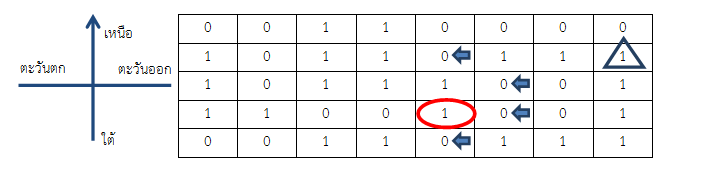
\includegraphics[width=1\textwidth]{../latex/img/1160/1160-1.png}
\end{figure}

ยิ่งไปกว่านั้น อินเดียนายังสนใจด้วยว่าทางเดินจากจุดเริ่มต้นไปถึงทางออกที่ใกล้ที่สุดมี ระยะทางเท่าใด (ระยะทางนับจากจำนวนช่องที่เดินผ่าน) จากตัวอย่างเดิม ถ้าอินเดียนาระเบิดกำแพงที่ช่อง ณ ตำแหน่งแถวที่สอง หลักที่ห้า หรือ ตำแหน่งแถวที่สาม หลักที่หก จะทำให้ได้ทางเดินที่ใกล้ที่สุดด้วย คือได้ทางเดินที่ผ่านจำนวนช่องทั้งหมด $6$ ช่อง (นับช่องที่จุดเริ่มต้นและสิ้นสุดและช่องที่เป็นกำแพงที่ถูกระเบิดด้วย)



\bigskip
\underline{\textbf{โจทย์}}   จงเขียนโปรแกรมที่มีประสิทธิภาพในการหาจำนวนช่องของกำแพงที่อินเดียนาสามารถทำ การระเบิดเพื่อนำอินเดียนาไปสู่ทางออกได้ รวมทั้งหาระยะทางเดินที่สั้นที่สุดจากจุดเริ่มต้นไปจนถึงทางออก


\InputFile

\textbf{บรรทัดแรก} ระบุค่า $M$ และ $N$ ซึ่งแทนจำนวนแถวและจำนวนหลักของเขาวงกตตามลำดับ โดยที่ $1 \leq M,N \leq 150$ โดย $M$ และ $N$ ถูกคั่นด้วยช่องว่าง

\textbf{บรรทัดที่สอง} ระบุแถว $r_s$ และหลัก $c_s$ ของช่องที่อินเดียนาเริ่มต้น โดยที่ $1 \leq r_s \leq M$ และ $1 \leq c_s \leq N$ โดย $r_s$ และ $c_s$ ถูกคั่นด้วยช่องว่าง

\textbf{บรรทัดที่สาม} ระบุแถว $r_e$ และหลัก $c_e$ ของช่องที่เป็นทางออก โดยที่ $1 \leq  r_e \leq M$ และ $1 \leq c_e \leq N$ โดย  $r_e$ และ $c_e$ ถูกคั่นด้วยช่องว่าง

\textbf{บรรทัดที่ $4$ ถึง $M+3$} ในแต่ละบรรทัดจะประกอบไปด้วยเลขจำนวน $N$ ตัว แต่ละตัวคั่นด้วยช่องว่าง โดยเลขศูนย์แทนกำแพง และเลขหนึ่งแทนทางเดิน บรรทัดแรกใน $M$ บรรทัด นี้บอกลักษณะช่องของแถวแรกในเขาวงกต (แถวแรกคือแถวที่อยู่ทางเหนือสุด) เรียงจากหลักทางทิศตะวันตกไปตะวันออก (หลักแรกคือหลักทางทิศตะวันตก) บรรทัดถัดมาบอกลักษณะของแถวที่สอง และเป็นเช่นนี้ไปเรื่อย ๆ จนครบ $M$ บรรทัด


\OutputFile

\textbf{บรรทัดแรก} ระบุจำนวนช่องกำแพงที่อินเดียนาสามารถวางระเบิดและพาอินเดียนาไปถึงทางออกได้

\textbf{บรรทัดที่สอง} ระบุระยะทางที่น้อยที่สุดที่อินเดียนาสามารถเดินเพื่อไปถึงทางออก โดยระยะทางคือจำนวนช่องที่อินเดียนาเดินผ่านทั้งหมด ซึ่งนับรวมช่องที่เป็นจุดเริ่มต้นและจุดสิ้นสุด พร้อมทั้งนับรวมช่องกำแพงที่อินเดียนาระเบิดด้วย

\Examples

\begin{example}
\exmp{5 8
4 5
2 8
0 0 1 1 0 0 0 0
1 0 1 1 0 1 1 1
1 0 1 1 1 0 0 1
1 1 0 0 1 0 0 1
0 0 1 1 0 1 1 1}{4
6}%
\end{example}

\begin{example}
\exmp{6 8
1 4
2 7
0 0 1 1 0 0 0 0
1 0 1 1 0 0 1 1
1 0 1 1 1 0 0 1
1 1 0 0 1 0 0 1
0 0 1 1 0 1 1 1
0 1 0 1 1 1 1 1}{4
13}%
\end{example}


\Source

การแข่งขันคอมพิวเตอร์โอลิมปิกระดับชาติครั้งที่ 8 (SUTOI8)


\end{problem}

\end{document}